\documentclass{article}
% Commands
\newcommand{\ASSNMT}{Project Necromancer}
\newcommand{\CLASS}{Design Document}
\newcommand{\Footer}{Grand Valley State University}

\newcommand{\DATE}{April 2015}

% Packages
\usepackage[utf8]{inputenc}
\usepackage[T1]{fontenc}
\usepackage{lmodern}
% \usepackage{pdflscape}
\usepackage{geometry}
\usepackage[usenames,dvipsnames]{xcolor}
\usepackage{graphicx}
\usepackage{mathtools}
\usepackage{caption}
\usepackage{amssymb}
%\usepackage{pdfpages}
%\usepackage{hyperref}
\usepackage[pdftex, pdfborderstyle={/S/U/W 0}]{hyperref} % this disables the boxes around links]
% Packages for Pygments
%\usepackage{fancyvrb}
%\usepackage{color}

% For making floating objects (tables) not be repositioned
% use "H" modifier for tables (\begin{table}[H])
\usepackage{float}
%\usepackage{subfigure}
% \restylefloat{table}
% For text subscripts
% \usepackage{fixltx2e}

% \usepackage{listings}
% \usepackage{color}

\usepackage{enumitem}
% For requirements list
%\renewcommand*{\theenumi}{\thesection.\arabic{enumi}}
%\renewcommand*{\theenumii}{\theenumi.\arabic{enumii}}
%\setlist[enumerate,1]{label={\textbf{Requirement \thesubsection.\arabic*}}}

\usepackage{fancyhdr}

% \definecolor{dkgreen}{rgb}{0,0.6,0}
% \definecolor{gray}{rgb}{0.5,0.5,0.5}
% \definecolor{mauve}{rgb}{0.58,0,0.82}

% \lstset
% {
%   frame=single,
%   frameround=tttt,
%   language=C,
%   numberstyle=\tiny\color{gray},
%   keywordstyle=\color{blue},
%   commentstyle=\color{dkgreen},
%   stringstyle=\color{mauve},
%   tabsize=3,
%   breaklines=true,
%   basicstyle={\small\ttfamily},
%   xleftmargin=\fboxsep,
%   xrightmargin=-\fboxsep,
%   numbers = left,
%   stepnumber = 5,
%   firstnumber = 1
% }

% \newcommand{\namesigdate}[2][5cm]{%
%   \begin{tabular}{@{}p{#1}@{}}
%     #2 \\[2\normalbaselineskip] \hrule \\[0pt]
%     {\small \textit{Signature}} \\[2\normalbaselineskip] \hrule \\[0pt]
%     {\small \textit{Date}}
%   \end{tabular}
% }


\begin{document}
% =====----- Initial Set Up -----=====
% Title Page
\newgeometry{top=2cm,left=1cm,bottom=1cm,right=1cm}
\begin{flushleft}
\pagenumbering{gobble}

\textsc{\LARGE \bfseries \ASSNMT}\\

\textsc{\Large \CLASS}\\[0.2cm]
\linethickness{0.5mm}
{\color{ForestGreen}\line(1,0){350}} \\ [2.0cm]

\begin{flushleft} \large
\begin{tabular}{lll}
  Sponsored By: & The Rainforest Connection (RFCx) 
\includegraphics[height=0.4cm]{rfcxlogo} & \\
                &               & \\
  Submitted By: & Joe Gibson    & \href{mailto:gibsjose@mail.gvsu.edu}{gibsjose@mail.gvsu.edu}\\
              & David Adlof     & \href{mailto:adlofd@mail.gvsu.edu}{adlofd@mail.gvsu.edu}\\
              & Kalee Stutzman  & \href{mailto:stutzmak@mail.gvsu.edu}{stutzmak@mail.gvsu.edu}\\
              & Jesse Millwood  & \href{mailto:millwooj@mail.gvsu.edu}{millwooj@mail.gvsu.edu}\\
\end{tabular}

\bigskip

\bigskip
Date Submitted: \DATE
\end{flushleft}

\bigskip
{\color{ForestGreen}\line(1,0){350}} \\ [2.0cm]
\section*{Executive Summary}
Software, electrical, and hardware enhancements to Rainforest Connection’s currently used device are proposed in this paper. The electrical enhancements include the addition of a new PCB that contains power regulation and battery charging circuitry, along with current, voltage, temperature, and humidity sensors. The software enhancements include sending sensor measurements to an Android cellphone. The hardware enhancements may include the design of a new enclosure with the intended climate taken into consideration. The point of this project is not to entirely redesign the existing device but rather to provide modular enhancements and improvements to specific components outlined in the rest of this document.


\section*{Keywords}
Rain forest, Recycling, RFCx, Rainforest Connection, cellphone, Android, logging

\vfill

% Bottom of the page
\begin{center}
{\large \Footer}
\end{center}
\begin{figure}[H]
  \centering
  
\includegraphics[width=.1\textwidth]{small_gvsu}
\end{figure}
\end{flushleft}
\restoregeometry
\newpage
% Define Page Geometry for rest of report
{\newgeometry{left=0.8in, right=0.8in, top=1in, bottom=1in}
% Page Numbers
\pagenumbering{arabic}
\pagestyle{fancy}
\fancyhf{}
\lhead{\ASSNMT}
\rfoot{Page \thepage}
% No paragraph indents
\setlength{\parindent}{0cm}
% =====----- Rest of Report -----=====
\newpage
\section{Introduction and Design Background}
Rainforest Connection (RFCx) is a non-profit organization that is dedicated to stopping illegal logging and deforestation in rainforests throughout the world. The destruction of tropical rainforests is a leading cause of CO2 emission, and much of it is caused by illegal activities. RFCx combats illegal logging by using re-purposed cell-phones strategically placed in trees in remote areas. These cell phones listen and record audio streams at all times, using their data connection to periodically send audio data to the RFCx server, where it is processed. Digital signal processing algorithms are used to detect the sound of chainsaws and engines, because the sheer size of the area covered by a single human makes it impractical, if not impossible, to properly monitor the forests for illegal activities without the aid of technology. If a chainsaw is detected, a real-time alert is sent to pre-existing ground patrols, who can react to the situation and combat the threat. In addition to man-made sounds, the RFCx platform is also used to record the sounds of animals in the forest. These sounds can be used to gain information about certain species of animals and are open to anyone to use and analyze.

RFCx Project Necromancer is a project involving the design of new hardware, as well as upgrades to the existing hardware. The principal objective is to merge all of the external electronics into a custom printed circuit board. This involves integrating the regulation circuitry, photovoltaic battery charge controller, sensors (temperature, power, etc.), microcontroller, and other supporting electronics into a single board. Diagnostic features like monitoring temperature, humidity, and power statistics and sending diagnostic information to the phone will be performed as well.

On the PCB, an ATMega328P microcontroller will be used. An SPV1040 Max Point Power Tracker (MPPT) will be used to obtain the maximum power from the solar panels and to efficiently charge the Lithium-Ion batteries. Current and voltage measurements on both the solar panel inputs as well as the output to the batteries will be measured by using an external ADC. The ADC chosen is a low-power TI ADS1015, which has four single-ended analog inputs, and draws as little as 150uA of current even in constant mode. Two options are considered for temperature, one also providing humidity measurements. The single temperature sensor is the NXT LM75BD, which is a super low power temperature sensor with an accuracy of $\pm2^{\circ}C$, communicating over I2C. The LM75BD uses less around 300uA during peak transmission, and costs under \$1. The combined temperature and humidity sensor is the Honeywell HIH6130, which is a low-power sensor with 14-bit resolution for both humidity and temperature, low-current operation, from 1uA in sleep mode to under 1mA worst case draw. The HIH6130 chip also has its own internal ADC, EEPROM, and oscillator, but costs nearly \$14. All three ICs communicate with the microcontroller via the I2C protocol. For communication with the Android phone, the ATMega328P serial port will be interfaced through FTDI to an on-board USB connector.

On the phone, the RFCx Sentinel App monitors the incoming diagnostics, displaying them to a screen, logging them to a file, and possibly transmitting them along with the audio data to the server.

\begin{figure}[H]
  \centering
  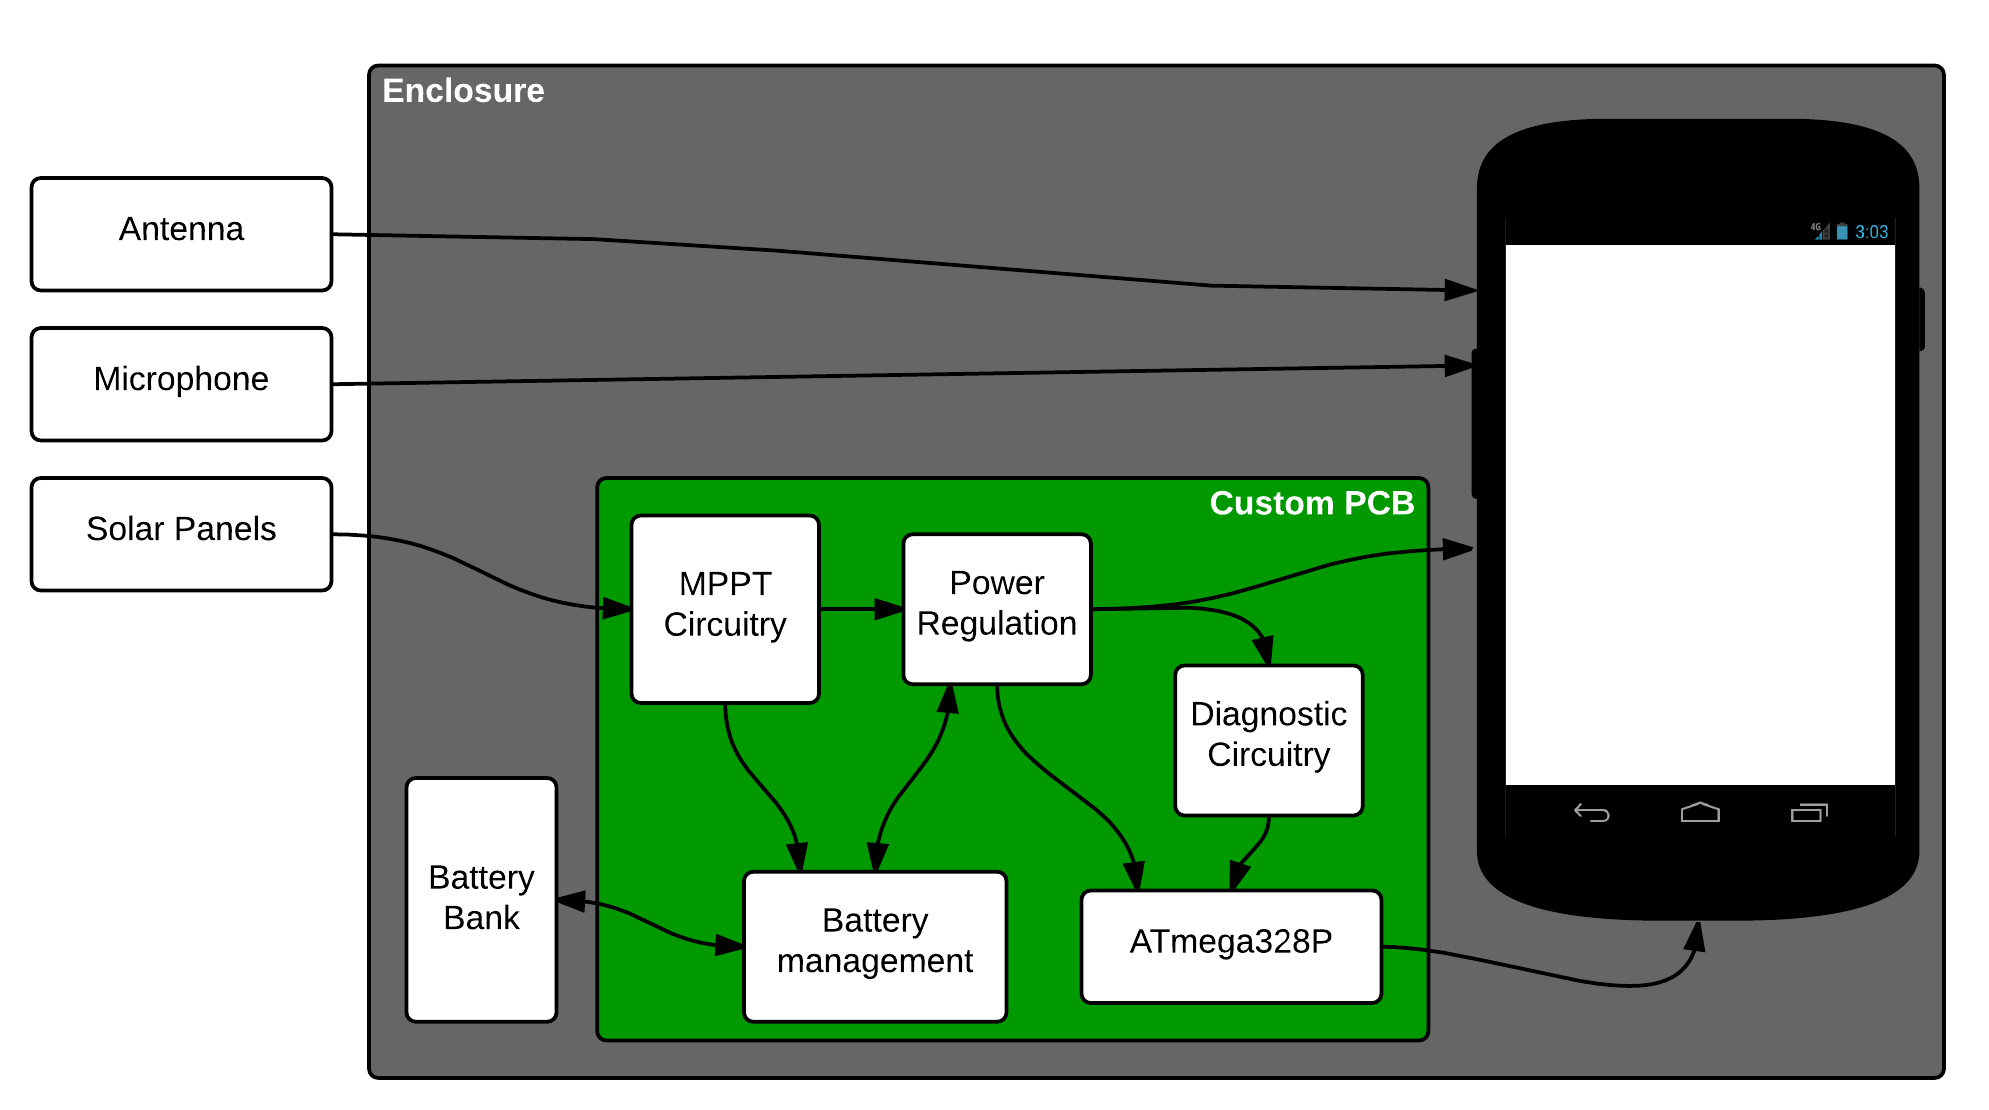
\includegraphics[width=0.8\textwidth]{Highlevel}
  \caption{High Level Diagram}
  \label{fig:hldia}
\end{figure}

\begin{figure}[H]
	\centering
	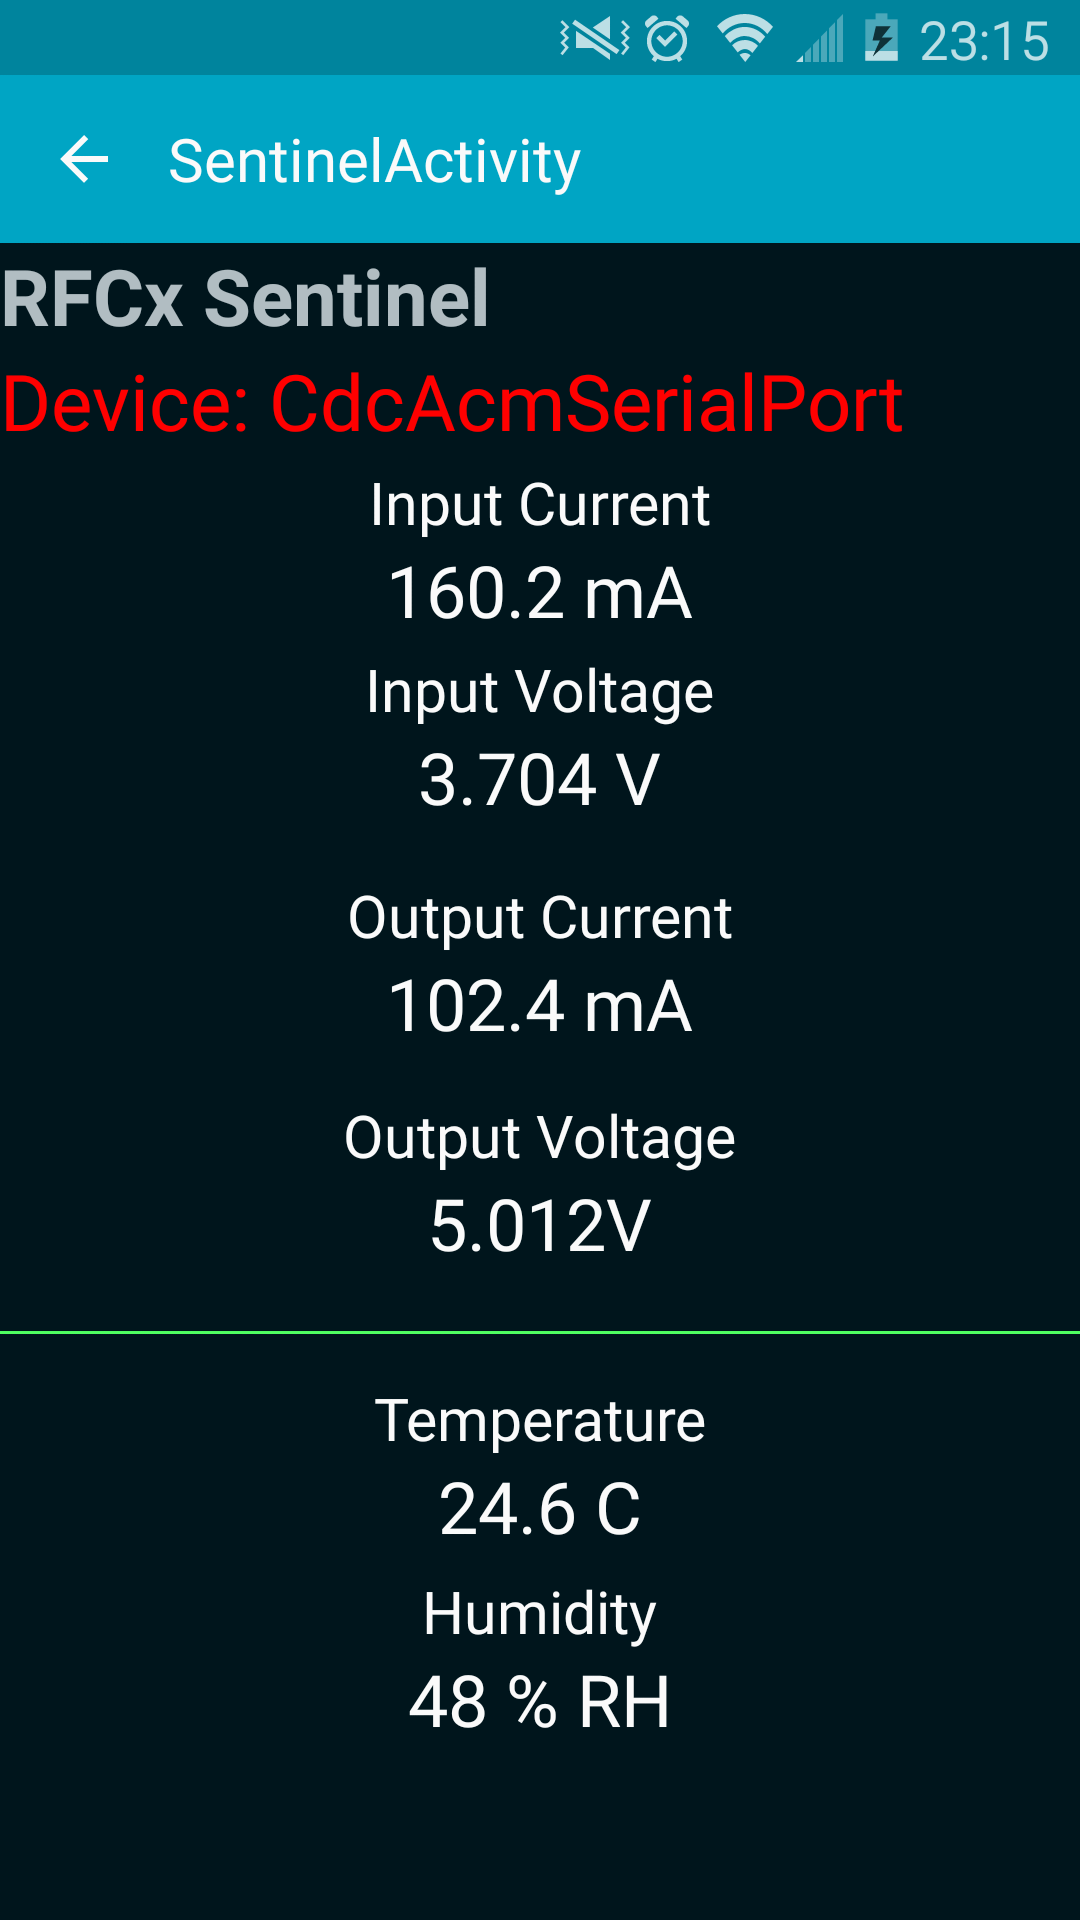
\includegraphics[width=0.4\textwidth]{RFCxSentinelScreenshot}
	\caption{Actual RFCx Sentinel App Screenshot}
	\label{fig:sentscrn}
\end{figure}
\section{Requirements and Functional Specifications}
\subsection{External Interfaces Requirements}
This section addresses the requirements of the enhanced device pertaining to its external interfaces. External interfaces are defined as components of the device interacting with something outside of the device enclosure.
\subsubsection{Hardware}
\begin{enumerate}[align=left,leftmargin=*, labelindent= 0em, label=\textbf{Requirement \thesubsubsection.\arabic*.}, itemindent=0em]

\item \label{HWa} The device shall not exceed the existing power consumption and should reduce power consumption by at least 10\%.
\item \label{HWb} The interface with the phone shall consist of a USB connection for power and data, a microphone connection via the standard audio jack, and a connection to the external antenna.
\item \label{HWc} The interface with the phone shall consist of a USB connection for power and data, a microphone connection via the standard audio jack, and a connection to the external antenna.
\item \label{HWd} Shielding techniques should be investigated to reduce the GSM audio interference noted by Topher White in the audio recordings.
\item \label{HWe} The microphone shall be interfaced via the standard audio jack on the Android phone.
\item \label{HWf} Camouflage color scheme may be used to conceal the device from loggers.  Additional camouflage features may be added so long as those features do not cover the solar panels.
\item \label{HWg} A simple assembly process shall be well documented with illustrations.

\baselinestretch
To verify \ref{HWg}. a sample group of people with varying skill levels will be asked to provide feedback on the assembly process and will be timed.

\item \label{HWh} The assembly and installation documentation may be translated into Spanish, French, and/or Portuguese.
\end{enumerate}
\subsubsection{Software}
\begin{enumerate}[align=left,leftmargin=*, labelindent= 0em, label=\textbf{Requirement \thesubsubsection.\arabic*.}, itemindent=0em]
\item \label{SWa} The algorithm used to compress the audio signal may be compared to other existing algorithms and may be changed as such depending on the outcomes of comparative testing.

\baselinestretch
To verify \ref{SWa}, audio will be recorded and compressed using multiple algorithms including the current algorithm. An infographic hosted on RFCx’s website, shown in Figure 2 illustrates the flow of data that is collected from the phone and analyzed on the server.
\end{enumerate}

\subsection{Internal Device Requirements}
This section addresses the requirements of the enhanced device pertaining to its internal interfaces and software. Internal here is defined as anything inside of the device enclosure.
\subsubsection{Hardware}
\begin{enumerate}[align=left,leftmargin=*, labelindent= 0em, label=\textbf{Requirement \thesubsubsection.\arabic*.}, itemindent=0em]
\item \label{HW1}The PCB shall consist of battery management circuitry, the power regulation circuitry, power interface to the phone, power monitoring circuitry, as well as the microphone interface.

\baselinestretch
To verify \ref{HW1}, SPICE will be used to simulate the power charging circuitry to obtain power consumption and efficiency calculations. The manufactured and assembled board will then be subjected to a load test in a lab setting.

\item \label{HW2}The device shall use the existing external microphone and antennae
\item \label{HW3}There should be a low power microcontroller included on the PCB that communicates with the Android phone. This will be used to monitor power consumption and provide external control of peripherals through the Android Debug Bridge protocol over USB. Extra general purpose IO pins of the microcontroller should be easily accessible for interfacing with future hardware.

\baselinestretch
To verify \ref{HW3}, simple packets will be sent from the microcontroller to the phone. These packets can be verified with debug tools or simple programs on the microcontroller and the phone. A debug serial port may be included as a peripheral to the microcontroller to aid in debugging. Any analog values read by the microcontroller will be verified with shop equipment.

\item \label{HW4} The monetary cost of the device, not including the solar panels, shall not exceed 25\% more than the current device cost, also not including the solar panels. The current cost of the solar panels has been quoted at \$200 and the rest of the device has been quoted at \$200. Increases in monetary cost above the current cost and below 125\% of the current cost are for enhancements in functionality (i.e. the PCB, etc.) and reductions in assembly time.

\end{enumerate}
\subsubsection{Software}
\begin{enumerate}[align=left,leftmargin=*, labelindent= 0em, label=\textbf{Requirement \thesubsubsection.\arabic*.}, itemindent=0em]
\item \label{SW1}The microcontroller software should be capable of bi-directional communication between itself and the Android phone.
\item \label{SW2}The microcontroller software should be capable of communicating power usage diagnostics to the phone over the ADB protocol.
\item \label{SW3}An Android companion application may be capable of reporting power diagnostics from the microcontroller for testing and debugging.
\item \label{SW4}There shall be a header on the PCB to program to reprogram the microcontroller.
\end{enumerate}



\end{document}

% ======== For Reference =============
% H parameter for the figure environment
% keeps it from floating
\begin{figure}[H]
	\centering
	\includegraphics[width=0.8\textwidth]{FIG2_1b}
	\caption{Convolution of Identical Unit Step Sequences}
	\label{fig:21b}
\end{figure}
% To turn off caption numbering place this:
%\captionsetup[figure]{labelformat=empty}
% Before the figure, To turn back on:
%captionsetup[figure]{labelformat=default}
\begin{equation}
	\begin{array}{rcl}
	y[n] &=& 0.5x[n]+x[n-1]+2x[n-2]\\
	y[n] &=& 0.8y[n-1]+2x[n]\\
	y[n]-0.8y[n-1] &=& 2x[n-1]
	\end{array}
\end{equation}

\begin{subequations}
	\begin{align}
		h[n] &= 2\delta[n+1]-2\delta[n-1]\\
		x[n] &= \delta[n] + \delta[n-2]
	\end{align}
\end{subequations}

% Resize used to make table width of text, may be omitted
\begin{table}[h]
\resizebox{\textwidth}{!}{
\centering
\begin{tabular}{|c|c|c|c|}
\hline
Case & $Z_c$          & $l$           & $c$       \\ \hline
1    & $110.9 \Omega$ & 0.593 $\mu H$ & 0.048 nF  \\ \hline
2    & $171.3 \Omega$ & 0.803 $\mu H$  & 27.408 pF \\ \hline
3    & $327.3 \Omega$ & 1.102 $\mu H$  & 10.294 pF \\ \hline
\end{tabular}}
\caption{Calculated Parameters}
\label{tbl:calcd}
\end{table}

% Code Snippet:
\begin{lstlisting}[language=C,label=lala,caption=this thing]
  code snippet
\end{lstlisting}

% bulleted list
\begin{itemize}
\item this is an item
\end{itemize}

\renewcommand*\contentsname{ }
\tableofcontents
\listoffigures

